\documentclass[t,usenames,dvipsnames]{beamer}
\usetheme{Copenhagen}
\setbeamertemplate{headline}{} % remove toc from headers
\beamertemplatenavigationsymbolsempty

\usepackage{amsmath, sfmath, tikz, xcolor, pgfplots, array}
\pgfplotsset{compat = newest}
\usetikzlibrary{arrows.meta, calc, decorations.pathreplacing}
\everymath{\displaystyle}

\title{Polynomials and Their Graphs}
\author{}
\date{}

\AtBeginSection[]
{
  \begin{frame}
    \frametitle{Table of Contents}
    \tableofcontents[currentsection]
  \end{frame}
}

\begin{document}

\maketitle

\begin{frame}{Polynomial Functions}
A \alert{polynomial function} is a function in the form
\[ f(x) = a_nx^n + a_{n-1}x^{n-1} + \cdots + a_2x^2 + a_1x + a_0 \]

where $a_0, a_1, \dots , a_n$ are real numbers and $n \geq 1$ is a natural number. \newline\\

The \textbf{domain} of a polynomial function is $(-\infty, \infty)$
\end{frame}

\section{Determine if a function is a polynomial}

\begin{frame}{Graphs of Polynomial Functions}
Graphs of polynomials are {\color{blue}\textbf{smooth}} and {\color{red}\textbf{continuous}}.   \newline\\  \pause

By ``smooth", we mean that there are no ``corners" or ``cusps" (sharp points) on the graph. \newline\\ \pause

By ``continuous" we mean that there are no ``breaks" or ``holes" in the graph (i.e. you can draw it without lifting the pencil off the paper.)
\end{frame}

\begin{frame}{Example 1}
Determine if each of the following are polynomials. \newline\\
(a) \quad $g(x) = \frac{4+x^3}{x}$  \newline\\  \pause
Not a polynomial. The domain is not $(-\infty, \infty)$ \newline\\  \pause
(b) \quad $p(x) = \frac{4x+x^3}{x}$ \newline\\  \pause
Not a polynomial. The domain is not $(-\infty, \infty)$ 
\end{frame}

\begin{frame}{Example 1}
(c) \quad $q(x) = \frac{4x+x^3}{x^2+4}$ 
\begin{align*}
    \onslide<2->{\frac{4x+x^3}{x^2+4} &= \frac{x(4+x^2)}{x^2+4}} \\[8pt]
    \onslide<3->{&=x} 
\end{align*}
\onslide<4->{Is a polynomial.} \newline\\
\onslide<5->{
\begin{itemize}
    \item Original domain is $(-\infty, \infty)$ \newline\\
    \item Can be written as $q(x) = 1x^1$
\end{itemize}
}
\end{frame}

\begin{frame}{Example 1}
(d) \quad $f(x) = \sqrt[3]{x}$  \newline\\  \pause
Not a polynomial.   \newline\\  \pause
\[ f(x) = \sqrt[3]{x} = x^{1/3} \]  \newline\\ \pause
1/3 is not a natural number
\end{frame}

\begin{frame}{Example 1}
(e) \quad $h(x) = |x|$ \newline\\ \pause
Not a polynomial.   \newline\\  \pause
Could only be written in piecewise form
\[
f(x) = 
\begin{cases}
x &\text{ if } x \geq 0 \\
-x &\text{ if } x < 0 \\
\end{cases}
\]
\end{frame}

\begin{frame}{Example 1}
(f) \quad $z(x) = 0$    \newline\\  \pause
Is a polynomial.    \newline\\  \pause
\begin{itemize}
    \item Can be written as $z(x) = 0x^n + 0x^{n-1} + \cdots + 0$ \newline\\
    \item Domain is $(-\infty, \infty)$
\end{itemize}
\end{frame}

\section{Find the degree, leading term, leading coefficient, and constant term of a polynomial}

\begin{frame}{Polynomial Vocabulary}
    For $f(x) = a_nx^n + a_{n-1}x^{n-1} + \cdots + a_2x^2 + a_1x + a_0$:    \newline\\
    \begin{itemize}
        \item<+-> $n$ is the \alert{degree} of the polynomial. \newline\\
        \item<+-> The term $a_nx^n$ is the \alert{leading term} of the polynomial.    \newline\\
        \item<+-> $a_n$ is the \alert{leading coefficient} of the polynomial.  \newline\\
        \item<+-> $a_0$ is the \alert{constant term} of the polynomial. \newline\\
    \end{itemize}
    \onslide<6->{If $f(x) = a_0$, and $a_0 \neq 0$, then $f$ has degree 0.} \newline\\
    \onslide<7->{If $f(x) = 0$, then $f$ has no degree}
\end{frame}

\begin{frame}{Example 2}
Find the degree, leading term, leading coefficient, and constant term of the following polynomials. \newline\\
(a) \quad $f(x) = 4x^5 - 3x^2 + 2x - 5$ \newline\\  \pause
\begin{itemize}
    \item<+-> Degree is 5 \newline\\
    \item<+-> Leading term is $4x^5$ \newline\\
    \item<+-> Leading coefficient is 4 \newline\\
    \item<+-> Constant is $-5$
\end{itemize}
\end{frame}

\begin{frame}{Example 2}
(b) \quad $g(x) = 12x + x^3$ \pause
\[ g(x) = x^3 + 12x \] \pause
\begin{itemize}
    \item<+-> Degree is 3 \newline\\
    \item<+-> Leading term is $x^3$ \newline\\
    \item<+-> Leading coefficient is 1 \newline\\
    \item<+-> Constant is $0$
\end{itemize}
\end{frame}

\begin{frame}{Example 2}
(c) \quad $h(x) = \frac{4-x}{5}$ \pause
\[ h(x) = \frac{4}{5}-\frac{1}{5}x = -\frac{1}{5}x + \frac{4}{5} \]   \pause
\begin{itemize}
    \item<+-> Degree is 1 \newline\\
    \item<+-> Leading term is $-\frac{1}{5}x$ \newline\\
    \item<+-> Leading coefficient is $-\frac{1}{5}$ \newline\\
    \item<+-> Constant is $\frac{4}{5}$
\end{itemize}
\end{frame}

\begin{frame}{Example 2}
(d) \quad $p(x) = (2x-1)^3(x-2)(3x+2)$  
\begin{align*}
    \onslide<2->{p(x) &= (2x)^3(x)(3x) + \text{ other terms } + (-1)^3(-2)(2)} \\[6pt]
    \onslide<3->{p(x) &= 8x^3(x)(3x) + \text{ other terms } + (-1)(-2)(2)} \\[6pt]
    \onslide<4->{p(x) &= 24x^5 + \text{ other terms } + 4}
\end{align*} 
\begin{itemize}
    \item<5-> Degree is 5 \\[6pt]
    \item<6-> Leading term is $24x^5$ \\[6pt]
    \item<7-> Leading coefficient is $24$ \\[6pt]
    \item<8-> Constant is $4$
\end{itemize}
\end{frame}

\section{Determine the end behavior of a polynomial}

\begin{frame}{End Behavior}
The \alert{end behavior} of a function refers to what is happening to the output values the further the graph of the function heads left and right.  \newline\\ \pause

In other words, what is happening to your $y$-coordinates the further $x$ goes to $\infty$ or to $-\infty$?
\end{frame}

\begin{frame}{End Behavior of Polynomials}
\textsc{Investigation:} \newline\\
What is the end behavior of
\[
f(x) = ax^n
\]

when $a$ is a positive real number and $n$ is an odd integer?    \newline\\ \pause

As $x \to -\infty, \, f(x) \to -\infty$ and \\
As $x \to \infty, \, f(x) \to \infty$   \newline\\ \pause

We would say that
\[
\lim_{x \to -\infty} f(x) = -\infty \quad \text{and} \quad \lim_{x \to \infty} f(x) = \infty
\]
\end{frame}

\begin{frame}{End Behavior of Polynomials}
\textsc{Investigation:} \newline\\
What is the end behavior of
\[
f(x) = ax^n
\]

when $a$ is a negative real number and $n$ is an odd integer?    \newline\\ \pause

As $x \to -\infty, \, f(x) \to \infty$ and \\
As $x \to \infty, \, f(x) \to -\infty$   \newline\\ \pause

We would say that
\[
\lim_{x \to -\infty} f(x) = \infty \quad \text{and} \quad \lim_{x \to \infty} f(x) = -\infty
\]
\end{frame}

\begin{frame}{End Behavior of Polynomials}
\textsc{Investigation:} \newline\\
What is the end behavior of
\[
f(x) = ax^n
\]

when $a$ is a positive real number and $n$ is an even integer?    \newline\\ \pause

As $x \to -\infty, \, f(x) \to \infty$ and \\
As $x \to \infty, \, f(x) \to \infty$   \newline\\ \pause

We would say that
\[
\lim_{x \to -\infty} f(x) = \infty \quad \text{and} \quad \lim_{x \to \infty} f(x) = \infty
\]
\end{frame}

\begin{frame}{End Behavior of Polynomials}
\textsc{Investigation:} \newline\\
What is the end behavior of
\[
f(x) = ax^n
\]

when $a$ is a negative real number and $n$ is an even integer?    \newline\\ \pause

As $x \to -\infty, \, f(x) \to -\infty$ and \\
As $x \to \infty, \, f(x) \to -\infty$   \newline\\ \pause

We would say that
\[
\lim_{x \to -\infty} f(x) = -\infty \quad \text{and} \quad \lim_{x \to \infty} f(x) = -\infty
\]
\end{frame}

\begin{frame}[c]{End Behavior Summary}
\begin{center}
\setlength{\extrarowheight}{6pt}
\begin{tabular}{c|c|c}
                        &   \textbf{Odd Degree}    &   \textbf{Even Degree} \\    \hline
    \textbf{L.C. is positive}    &   Down and Up   &   Up and Up     \\[3pt]  \hline
    \textbf{L.C. is negative}    &   Up and Down   &   Down and Down 
\end{tabular}
\end{center}
\end{frame}

\begin{frame}{Example 3}
Determine the end behavior of each of the following.    \newline\\
(a) \quad $f(x) = 4x^5 - 3x^2 + 2x - 5$ \newline\\  \pause
\onslide<2->{Positive lead coefficient, odd degree:} \newline\\
\onslide<3->{Down (as we go left) and up (as we go right)}
\onslide<4->{
\[ \lim_{x\to -\infty} f(x) = -\infty \quad \text{and} \quad \lim_{x\to \infty} f(x) = \infty \]}
\end{frame}


\begin{frame}{Example 3}
(b) \quad $g(x) = 12x + x^4$   
\onslide<2->{\[ g(x) = x^4 + 12x \]} 
\onslide<3->{Positive lead coefficient, even degree:} \newline\\
\onslide<4->{Up (as we go left) and up (as we go right)}
\onslide<5->{
\[ \lim_{x\to -\infty} g(x) = \infty \quad \text{and} \quad \lim_{x\to \infty} g(x) = \infty \]}
\end{frame}

\begin{frame}{Example 3}
(c) \quad $h(x) = \frac{4-x}{5}$   
\onslide<2->{\[ h(x) = -\frac{1}{5}x + \frac{4}{5} \]}
\onslide<3->{Negative lead coefficient, odd degree:} \newline\\
\onslide<4->{Up (as we go left) and Down (as we go right)}
\onslide<5->{
\[ \lim_{x\to -\infty} h(x) = \infty \quad \text{and} \quad \lim_{x\to \infty} h(x) = -\infty \]}
\end{frame}

\begin{frame}{Example 3}
(d) \quad $p(x) = 2x^7 - x^8$ 
\onslide<2->{\[ p(x) = -x^8 + 2x^7 \]}
\onslide<3->{Negative lead coefficient, even degree:} \newline\\
\onslide<4->{Down (as we go left) and Down (as we go right)}
\onslide<5->{
\[ \lim_{x\to -\infty} p(x) = -\infty \quad \text{and} \quad \lim_{x\to \infty} p(x) = -\infty \]}
\end{frame}

\section{Find the zeros of a polynomial}

\begin{frame}{Zeros of Polynomials}
The \alert{zeros} of a polynomial, $f(x)$, have a few aliases:  \newline\\
\begin{itemize}
    \item $x$-intercepts
    \item roots
    \item solutions to $f(x)=0$
\end{itemize}
\end{frame}

\begin{frame}{Example 4}
Find the zeros of each. \newline\\
(a) \quad $f(x) = 2x^4 + 7x^3 - 10x^2 - 33x + 18$   \newline\\
\begin{minipage}{0.6\textwidth}
\onslide<2->{
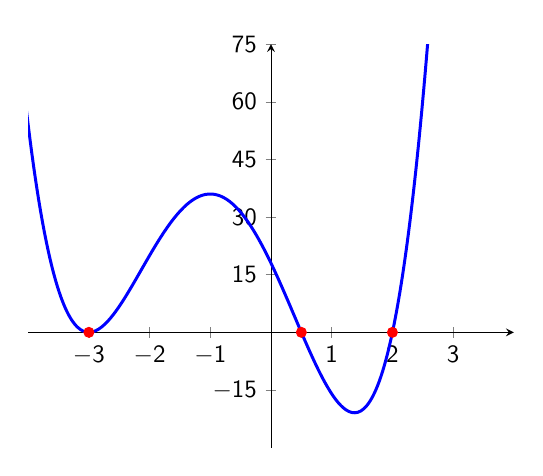
\begin{tikzpicture}[scale=0.9]
\begin{axis}[
axis lines = middle,
xmin = -4, xmax = 4,
ymin = -30, ymax = 75,
xtick = {-3,-2,...,3},
ytick = {-15,0,...,75}
]
\addplot[color=blue, very thick, samples=200, smooth] {2*x^4 + 7*x^3 - 10*x^2 - 33*x + 18};
\addplot[color=red, mark=*, only marks] coordinates {(-3,0) (0.5,0) (2,0)};
\end{axis}
\end{tikzpicture}}
\end{minipage}
\begin{minipage}{0.3\textwidth}
\onslide<3->{
$x$-intercepts: \newline\\
$(-3,0), \left(\frac{1}{2},0\right), (2,0)$}    \newline\\
\onslide<4->{Zeros: \newline\\
$x = -3, \frac{1}{2}, 2$} 
\end{minipage}
\end{frame}

\begin{frame}{Example 4}
(b) \quad $g(x) = (x-1)^3(5x+4)(x+7)^4$ \newline\\
\begin{align*}
\onslide<2->{x-1&= 0 & 5x+4&=0 & x+7&=0} \\[8pt]
\onslide<3->{x&=1 & x&=-\frac{4}{5} & x&=-7} \\
\end{align*}

\end{frame}

\end{document}
